\pdfminorversion=4
\documentclass[a4paper,12pt]{article}
\usepackage [spanish]{babel} 
\usepackage[utf8]{inputenc}
\usepackage{amsmath}
\usepackage{graphicx}
\usepackage{framed}
\usepackage{url}

\usepackage{fancyhdr}

\newcommand{\ihat}{\hat{\textbf{\i}}}
\newcommand{\jhat}{\hat{\textbf{\j}}}
\newcommand{\khat}{\hat{\textbf{k}}}
\newcommand{\vol}{\mathop{\ooalign{\hfil$V$\hfil\cr\kern0.08em--\hfil\cr}}\nolimits}

\graphicspath{{../img/}}
 
\pagestyle{fancy}
\setlength\headheight{1.5cm}
\fancyhf{}
\rhead{\includegraphics[width=3.0cm]{logo-mec.png}}
\lhead{\includegraphics[width=3.5cm]{logo-utfsm.png}}
\renewcommand{\footrulewidth}{0.5pt}
\rfoot{\tiny{Departamento de Ingenier\'ia Mec\'anica}}
\lfoot{\tiny{Universidad T\'ecnica Federico Santa Mar\'ia}}

\title{Clase 12 --- Aplicación de flujo potencial: aerodinámica.} 
\author{Christopher Cooper}
\date{}

\begin{document}
\maketitle
\begin{framed}

Objetivos:
\begin{itemize}
    \item Describir el mecanismo de separación de capa límite.
    \item Predecir la separación de la capa límite.
    \item Calcular la fuerza sobre cuerpos sumergidos no aerodinámicos.
\end{itemize}

Contenidos:
\begin{itemize}
    \item El mecanismo de separación de capa límite.
    \item El factor de forma y su influencia en la separación de la capa límite.
    \item El arrastre por fricción y el arrastre por presión.
    \item Coeficiente de arrastre.
\end{itemize}

Bibliografía:
\begin{itemize}
    \item Fox, R. W., Pritchard, P. J. y McDonald, A. T. (2009) Introduction to Fluid Mechanics. John Wiley \& Sons. Sección 9.6-9.7.
    \item White, F. M. (2008) Mecánica de Fluidos. McGraw-Hill. Sexta edición. Secciones 7.5-7.6.
\end{itemize}
\end{framed}

\section*{Separación de la capa límite}

Hasta ahora, todos nuestros análisis se han hecho bajo la suposición que la capa límite se mantiene pegada a la pared todo el tiempo, sin embargo, sabemos que esto no es así en la práctica. 
De hecho, ustedes fueron testigos de esto en el laboratorio 1.
Cuando midieron la presión alrededor de un cilindro, se dieron cuenta que en la zona posterior se perdía la tendencia tipo ``flujo potencial'' y la medición de presión se estancaba.
Esto ocurrió porque el flujo se separó de la pared del cilindro.

La razón por qué la capa límite se separa de la pared es la gradiente de presión.
Si la presión cae con $x$, se dice que hay una gradiente de presión favorable, ya que contrarresta la desaceleración del flujo debido al esfuerzo viscoso sobre la pared.
Por otra parte, si la presión aumenta con $x$, se dice que existe un gradiente de presión adverso, el cual desacelera el flujo, y puede generar la separación.
Un caso práctico es el flujo en un ducto divergente, donde la desaceleración del flujo genera un aumento de presión aguas abajo, y si el ángulo entre las paredes es muy grande, el flujo se puede separar.
Otro ejemplo es el flujo sobre un ala, donde al tener un ángulo de ataque muy alto, la gradiente de presión en la parte superior del ala se torna insostenible para la capa límite, y se separa.

\begin{figure}
\centering
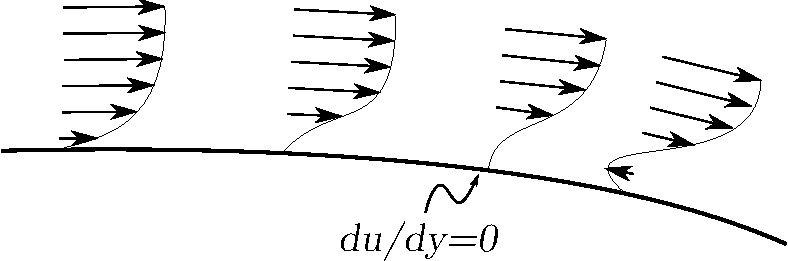
\includegraphics[width=0.8\textwidth]{clase12/separacion.pdf}
\caption{Mecanismo de separación de la capa límite.}
\label{fig:separacion}
\end{figure}

La Figura \ref{fig:separacion} muestra el mecanismo de separación de la capa límite.
El gradiente adverso de presión desacelera al flujo cerca de la pared, y lejos de la pared la inercia de $U_\infty$ arrastra la capa límite.
Por este efecto, la gradiente de velocidad sobre la placa disminuye, a tal punto que llega a ser cero ($\partial u/\partial y=0$).
Es en este punto donde se considera que el flujo se separa, ya que después de él hay un flujo en dirección contraria, que despega la capa límite.

\mbox{?`}Se acuerdan que el perfil de velocidad de una capa límite turbulenta tenía una gradiente de velocidad mayor que el perfil de Blasius cerca de la pared?
Si la gradiente es mayor, el mecanismo descrito por la Figura \ref{fig:separacion} demora más en separar el flujo (debe ``empujar'' el perfil desde una gradiente mayor).
Esta es la razón por la cual el flujo turbulento se demora más en separar.
De hecho, en las alas de aviones es muy común encontrar placas en la superficie que hacen las veces de generadores de turbulencia.
Al generar turbulencia, se retarda la separación, lo que es deseable para evitar el temido ``stall''.

\subsection*{Separación y el factor de forma}

Hasta ahora, cuando hemos hablado de la relación integral de von Kármán, solamente ha sido en el cotexto de un flujo a presión constante.
En el caso general, esta relación es
%
\begin{equation}\label{eq:integral_vK}
\tau_w = \rho U_\infty^2\frac{d\theta}{dx} + \rho(\delta^*+2\theta)U_\infty \frac{dU_\infty}{dx}.
\end{equation}
%
De hecho, si evalúan la Ec. \eqref{eq:integral_vK} para el caso particular donde la presión es constante (y, por ende, la velocidad $U_\infty$ es constante), llegamos a la expresión que vimos hace algunas clases.
Podemos adimensionalizar la Ec. \eqref{eq:integral_vK}, y reescribirla de la siguiente forma
%
\begin{equation}
\frac{\tau_w}{\rho U_\infty^2} = \frac{c_f}{2} = \frac{d\theta}{dx} + (H+2)\frac{\theta}{U_\infty} \frac{dU_\infty}{dx}.
\end{equation}
%
donde $H=\delta^*/\theta$ se conoce como el factor de forma.
El factor de forma es el mejor indicador de cuando va a ocurrir la separación. 
En el caso de flujo laminar, $H_\text{sep}=3.5-4$ al separarse la capa límite.
Si es turbulento, un valor típico es $H_\text{sep}=2.6$.
Como referencia, en una placa plana, $H_\text{lam} = 2.6$ si la capa límite es laminar, y $H_\text{turb} = 1.3$ si es turbulenta, por lo tanto, para la placa plana no ocurrirá separación.

\section*{Arrastre sobre cuerpos sumergidos}

En general, es más común encontrar cuerpos donde la capa límite se separa, lo cual complica mucho el cálculo de la fuerza sobre éste.
Cuando la capa límite se separa, ya no tenemos expresiones de $c_f$, y tenemos que usar coeficientes empíricos para obtener la fuerza.
La forma más fácil de analizar estos problemas es descomponiendo la fuerza (en verdad, el coeficiente de arrastre), en dos: arrastre por fricción y arrastre por presión
%
\begin{equation}
C_D = \frac{F_D}{\frac{1}{2}\rho U_\infty^2 A} = C_f + C_p,
\end{equation}
%
donde,
%
\begin{align}\label{eq:CfCp}
C_f & = \frac{F_f}{\frac{1}{2}\rho U_\infty^2 A}= \frac{1}{A}\int c_f dA = \frac{1}{\frac{1}{2}\rho U_\infty^2 A}\int\tau_wdA\nonumber\\
C_p & = \frac{F_p}{\frac{1}{2}\rho U_\infty^2 A}= \frac{1}{\frac{1}{2}\rho U_\infty^2 A}\int p dA.
\end{align}

\subsection*{Arrastre por fricción}
Este es el caso que ya hemos estado estudiando, donde el cuerpo está alineado con el flujo, y la capa límite no se separa.
Tengan en consideración que para que un cuerpo tenga arrastre por fricción solamente, no es necesario que sea una placa plana, más bien, en cualquier cuerpo aerodinámico donde no hay separación (por ejemplo, un perfil alar), la fuerza de arrastre es solamente por fricción.
Para encontrar expresiones para esta fuerza, solamente debemos integrar las expresiones para $c_f$ que hemos estudiado últimamente.
En el caso laminar, esto sería
%
\begin{align}
C_f &= \frac{1}{A}\int\frac{0.664}{\sqrt{Re_x}}dA = \frac{1}{bL} \frac{0.664}{\left(\frac{V}{\nu}\right)}\int_0^L \frac{1}{\sqrt{x}} b dx \nonumber\\
&= \frac{1}{L} \frac{0.664}{\left(\frac{V}{\nu}\right)} 2\sqrt{L} = \frac{1.33}{\sqrt{Re_L}}.
\end{align}

Por otra parte, para capa límite turbulenta, $c_f=0.0594/Re_x^{1/5}$, y si despreciamos el hecho que el principio de la placa tiene un régimen laminar:
%
\begin{align}\label{eq:Cf_turb}
C_f &= \frac{1}{A}\int\frac{0.0594}{Re_x^{1/5}}dA = \frac{0.0594}{bL}\left(\frac{\nu}{U_\infty}\right)^{1/5}\int_0^Lx^{-1/5}bdx \nonumber\\
&=\frac{0.0594}{L}\left(\frac{\nu}{U_\infty}\right)^{1/5}\frac{5}{4}L^{4/5} = \frac{0.0742}{Re_L^{1/5}}.
\end{align}

En la clase anterior, llegamos a la expresión $c_f=0.0594/Re_x^{1/5}$ asumiendo que el perfil de velocidades se comportaba como $\sim y^{1/7}$, y al hacer el símil con flujo en tubería utilizamos la fórmula de Blasius para el factor de fricción $f$. 
La fórmula de Blasius es empírica, y tiene límites de aplicabilidad (funciona para $Re_D <10^5$), y esta limitante se traspasa a la placa plana.
De hecho, la fórmula de la Ec. \eqref{eq:Cf_turb} funciona bien para $Re_L<10^7$, y $Re_L>5\cdot10^5$ (ya que ahí ocurre la transición a turbulencia).
Para $Re_L>10^9$, Schlichting propuso la siguiente relación
%
\begin{equation}
C_f = \frac{0.455}{\log^{2.58}_{10}Re_L}
\end{equation}

Una particularidad del flujo sobre una placa plana es que coexiste flujo laminar (al inicio de la placa) y flujo turbulento (aguas abajo).
Si la zona donde el flujo es laminar no es despreciable, la expresión de la Ec. \eqref{eq:Cf_turb} ya no es válida. 
En este caso, se hacen los siguientes ajustes:
%
\begin{align}
C_f &= \frac{0.0742}{Re_L^{1/5}} - \frac{1740}{Re_L} \text{ para $5\cdot10^{-5}<Re_L<10^7$}\nonumber\\
C_f &= \frac{0.455}{\log^{2.58}_{10}Re_L} - \frac{1610}{Re_L} \text{ para $5\cdot10^{-5}<Re_L<10^9$}
\end{align}

\subsection*{Arrastre por presión}

El caso contrario, un cuerpo que soporta arrastre por presión solamente es aquel donde el flujo se separa completamente, y no hay un arrastre por fricción en la dirección del flujo.
El caso canónico es la placa que se enfrenta perpendicular al flujo.
En este caso, hay una capa límite en la cara enfrentada al flujo, sin embargo, el flujo sobre esta placa es perpendicular al flujo principal, y no aporta al arrastre.
Si hacemos un análisis de contidad de movimeinto sobre un volumen de control que solamente encierre la placa (por lo tanto, no hay flujos entrando y saliendo del volumen de control), veremos que la fuerza neta sobre la placa es solamente debido a la presión, dejándonos con la segunda expresión en la Ec. \eqref{eq:CfCp}.

El arrastre por presión está generalmente relacionado con el área enfrentada al flujo.
En este sentido, el arrastre por presión de una placa circular de radio $R$ será el mismo que sobre una esfera de radio $R$. 
Esto ocurre porque las componentes de $p\mathbf{n}$ (donde $\mathbf{n}$ es normal a la superficie) que no están alineadas con el flujo generalmente se cancelan.

Es prácticamente imposible obtener una expresión analítica para la presión alrededor de un cuerpo con separación de capa límite. 
Es por esto que para encontrar valores de $C_p$ es necesario recurrir a herramientas computacionales, a diferencia del arrastre por fricción.

\subsection*{Arrastre por fricción y presión}

En general, el arrastre es por una combinación de $C_f$ y $C_p$.
Considerando que es imposible obtener valores para $C_p$ de manera analítica, utilizamos valores para $C_D$ empíricos para nuestro análisis.
Los valores de $C_D$ dependen de la geometría (esfera, semi-esfera, cilindro, placa, etc.), y se sacan de tablas (vean la tabla 9.3 del Fox).
Eso si, $C_D$ depende también del $Re$, sin embargo, las tablas solamente entregan información ``discreta'', complicando el análisis.
Un ejemplo de esto es la Figura \ref{fig:arrastre_esfera} (sacada de \url{http://www.aerospaceweb.org/question/aerodynamics/q0231.shtml}), que muestra el arrastre sobre una esfera (y un disco) con respecto al número de Reynolds.
%
\begin{figure}
\centering
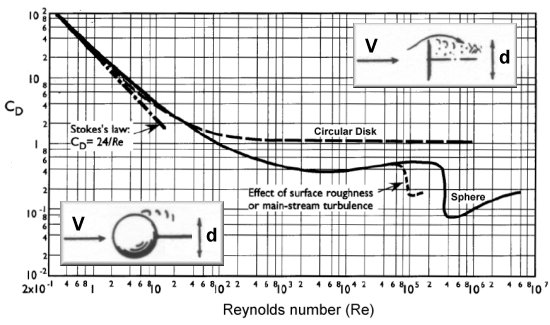
\includegraphics[width=0.7\textwidth]{clase12/arrastre_esfera.jpg}
\caption{Arrastre sobre una esfera y un disco.}
\label{fig:arrastre_esfera}
\end{figure}

Miremos la Figura \ref{fig:arrastre_esfera} y veremos algunas cosas interesantes.
Primero, vemos que para número de Reynolds muy bajo, la relación es prácticamente lineal.
De hecho, a Reynolds tan bajos el flujo no se separa, y despreciando los términos convectivos de la ecuación de Navier-Stokes podemos encontrar analíticamente que
%
\begin{equation}
F_D = 3\pi\mu U_\infty d
\end{equation}
%
y obtener la expresión para el coeficiente de arrastre 
%
\begin{equation}
C_D = \frac{24}{Re}
\end{equation}

Cuando el flujo se separa, perdemos esa relación lineal y pareciera ser que la relación entre $C_D$ y $Re$ se establiza, sin embargo, llega un punto donde $C_D$ cae drásticamente. 
Esta caída responde a la transición de la capa límite a turbulenta, que, como ya sabemos, demora más en separar, por lo tanto hay un área ``extra'' de no-separación que empuja la esfera hacia adelante, disminuyendo el arrastre.
Esto además confirma que en estos tipos de problema, el arrastre por presión es mayor que el arrastre por fricción, ya que la capa límite turbulenta tiene un perfil de velocidad con mayor gradiente, y por ende, mayor $\tau_w$.

Si la superficie es rugosa, la transición a turbulencia será antes, y $C_D$ caerá a un menor Reynolds.
Esto se ve en la Figura \ref{fig:arrastre_esfera} en la línea punteada.
Una aplicación de esto son las pelotas de golf, que tienen hoyitos para generar turbulencia y retrasar la separación, para así disminuir el arrastre.

En el caso que un cuerpo esté compuesto por partes de cuerpos de los cuales conocemos su arrastre, el arrastre total será la suma de cada una de las componentes.
Por ejemplo, un cilindro que está alineado con el flujo (con la sección transversal enfrentada a la velocidad externa), puede ser visto como la suma del flujo contra una placa circular más el flujo sobre una placa plana (el manto).

 
\end{document}
